The created system incorporates all the standard components needed for supervised machine learning, which were described in details in the theoretical section. First of all, to perform any task concerning image processing, a dataset of images is needed. In the thesis all images that are used were artificially generated. Thus, the first component of the system is an image generator. Having the dataset, the next step is preprocessing. Its main goal is to perform a division into superpixels, which limits the complexity of other processes. A separate component is responsible for this division. Having the dataset prepared there is a need to provide a method of transforming data from superpixels into meaningful features that are understandable by the algorithms used in the system. Hence, the next component performs feature selection. Chosen features are then extracted from each superpixel. As it has already been presented in the theoretical part, Conditional Random Fields are best modelled with the use of factor graphs, thus the next component performs factorisation. Factor graphs are composed of input nodes, one per each superpixel and output nodes. These are the main steps that are needed to provide input data for two main processes in the created semantic segmentation system which are parameter training and inference. Tough, for a part of the system in which a feature function is expressed in terms of the probability of occurrence given a set of features also another component is required. This component is aimed to provide an estimation of the probability distribution of features and labels that is needed to obtain the requested probability. The next component provides a supervised learning algorithm with the use of Stochastic Gradient Descent in order to adjust the weights of the system. Having a properly parametrised model it is possible to perform semantic image segmentation on an unknown image in the next component that conducts a process of maximum a posteriori inference. As it has been explained in the theoretical section, for Conditional Random Fields the most suitable inference algorithm is Loopy Belief propagation, which finds the most probable configuration of superpixel labels for a given image by means of the Min-Sum algorithm. Such configuration is exactly the result of semantic image segmentation. They way in which all components of the system are connected is presented in figure \ref{fig:component_diagram}.
\begin{figure}
    \centering
    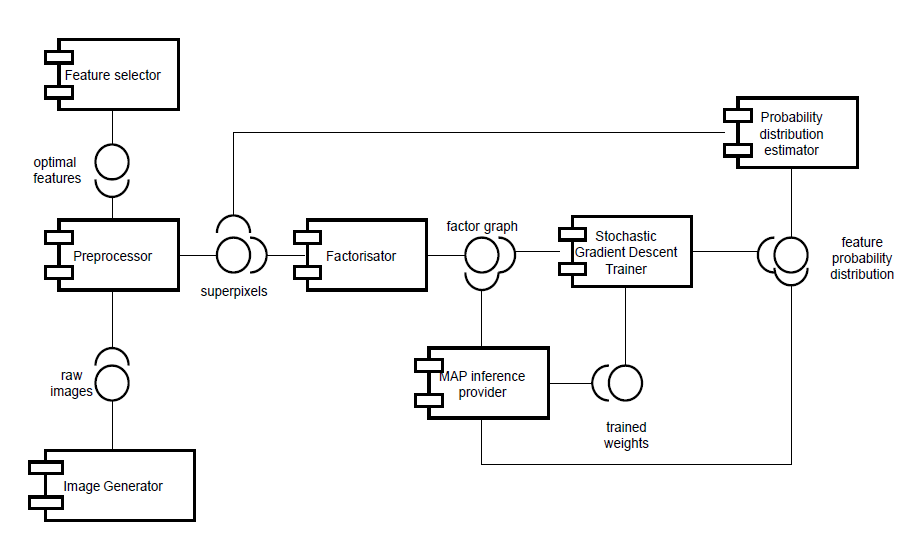
\includegraphics[width=\textwidth]{system_overview/component_diagram.png}
    \caption{Component diagram of the created semantic image segmentation system}
    \label{fig:component_diagram}
\end{figure}


